\documentclass[11pt]{article}

\usepackage[margin=1in]{geometry}
\usepackage{amsmath, amssymb, amsthm}
\usepackage{enumitem}
\usepackage{tikz}

\pagestyle{empty}

\begin{document}

\begin{center}
  {\Large\bfseries Weekly Assignment: Strong Induction,\\[2pt]
   Recursive Sequences, \& Recurrences\\[2pt]
   (Epp~5.4, 5.6, 5.7, \& 5.8)}
\end{center}

\bigskip

\noindent
Complete each of the following problems.  Show all work and justify your answers.

\bigskip

%% ─────────────────────────────────────────────
\noindent\textbf{Problem 1} (Epp 5.4 \#3). \;
Suppose that $c_0, c_1, c_2, \ldots$ is a sequence defined as
follows:
\[
  c_0 = 2,\quad c_1 = 2,\quad c_2 = 6,\qquad
  c_k = 3\,c_{k-3} \;\;\text{for every integer } k \ge 3.
\]
Prove that $c_n$ is even for each integer $n \ge 0$.

\bigskip

%% ─────────────────────────────────────────────
\noindent\textbf{Problem 2} (Epp 5.4 \#15). \;
Define the ``sum'' of one integer to be that integer itself.
Use strong mathematical induction to prove that for every
integer $n \ge 1$, any sum of $n$ even integers is even.

\bigskip

%% ─────────────────────────────────────────────
\noindent\textbf{Problem 3} (Epp 5.6 \#4). \;
Find the first four terms of the recursively defined
sequence:
\[
  d_k = k\,(d_{k-1})^2, \;\;\text{for every integer } k \ge 1,
  \qquad d_0 = 3.
\]

\bigskip

%% ─────────────────────────────────────────────
\noindent\textbf{Problem 4} (Epp 5.6 \#12). \;
Let $s_0, s_1, s_2, \ldots$ be defined by the formula
$\displaystyle s_n = \frac{(-1)^n}{n!}$
for every integer $n \ge 0$.  Show that this sequence
satisfies the following recurrence relation for every
integer $k \ge 1$:
\[
  s_k \;=\; \frac{-\,s_{k-1}}{k}\,.
\]

\bigskip

%% ─────────────────────────────────────────────
\noindent\textbf{Problem 5} (Epp 5.7 \#2\,b). \;
The formula
\[
  1 + r + r^2 + \cdots + r^n \;=\; \frac{r^{n+1} - 1}{r - 1}
\]
is true for every real number $r \ne 1$ and every integer
$n \ge 0$.  Use this fact to find a closed-form formula for:
\[
  3^{n-1} + 3^{n-2} + \cdots + 3^2 + 3 + 1,
\]
where $n$ is an integer with $n \ge 1$.

\bigskip

%% ─────────────────────────────────────────────
\noindent\textbf{Problem 6} (Epp 5.7 \#52). \;
A single line divides a plane into two regions.  Two lines
(by crossing) can divide a plane into four regions; three
lines can divide it into seven regions (see figure below).
Let $P_n$ be the maximum number of regions into which $n$
lines divide a plane, where $n$ is a positive integer.

\begin{center}
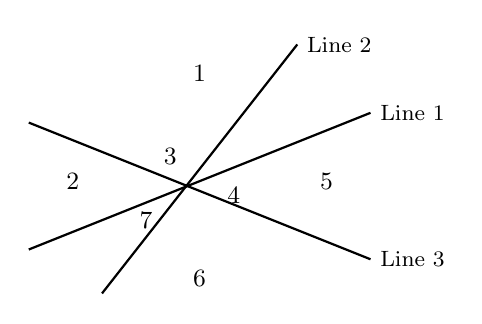
\begin{tikzpicture}[scale=0.62]
  % three lines in general position
  \draw[thick] (-3.5,-1.4) -- (3.5,1.4);   % Line 1
  \draw[thick] (-2,-2.3) -- (2,2.8);        % Line 2
  \draw[thick] (-3.5,1.2) -- (3.5,-1.6);    % Line 3
  % region labels
  \node at (0,2.2) {\small 1};
  \node at (-2.6,0) {\small 2};
  \node at (-0.6,0.5) {\small 3};
  \node at (0.7,-0.3) {\small 4};
  \node at (2.6,0) {\small 5};
  \node at (0,-2) {\small 6};
  \node at (-1.1,-0.8) {\small 7};
  % labels
  \node[right] at (3.5,1.4) {\footnotesize Line 1};
  \node[right] at (2,2.8) {\footnotesize Line 2};
  \node[right] at (3.5,-1.6) {\footnotesize Line 3};
\end{tikzpicture}
\end{center}

\begin{enumerate}[label=\textbf{\alph*.},itemsep=4pt]
  \item Derive a recurrence relation for~$P_k$ in terms
        of~$P_{k-1}$, for each integer $k \ge 2$.
  \item Use iteration to guess an explicit formula
        for~$P_n$.
\end{enumerate}

\bigskip

%% ─────────────────────────────────────────────
\noindent\textbf{Problem 7} (Epp 5.8 \#2). \;
Which of the following are second-order linear homogeneous
recurrence relations with constant coefficients?  For each,
briefly explain why or why not.

\begin{enumerate}[label=\textbf{\alph*.},itemsep=3pt]
  \item $a_k = (k-1)\,a_{k-1} + 2k\,a_{k-2}$
  \item $b_k = 2\,b_{k-1} + 7\,b_{k-2}$
  \item $c_k = 3\,c_{k-1} + 1$
  \item $d_k = 3\,d_{k-1}^{\,2} + d_{k-2}$
  \item $r_k = r_{k-2} - 6\,r_{k-3}$
  \item $s_k = s_{k-1} + 10\,s_{k-2}$
\end{enumerate}

\end{document}
